\documentclass[tikz, border=8pt]{standalone}
\usepackage{amsmath}
\usetikzlibrary{positioning, arrows.meta, calc}

\newcommand{\note}[1]{{\small\itshape #1}}
\newcommand{\boxtitle}[1]{{\bfseries #1}}
\newcommand{\eq}[1]{{\small $#1$}}

\begin{document}
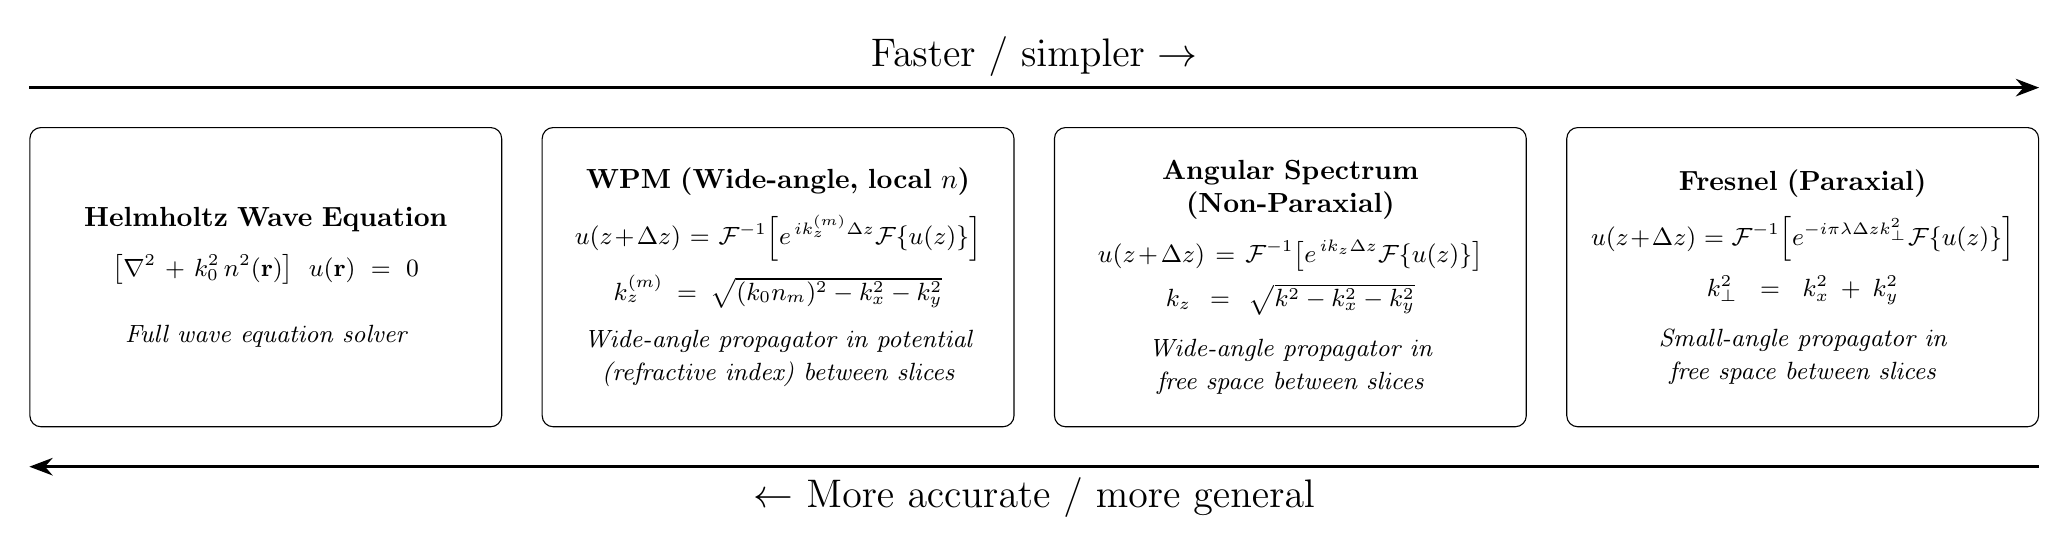
\begin{tikzpicture}[
    box/.style={
        rectangle,
        draw,
        rounded corners,
        align=center,% Changed from left to center for better balance
        text width=5.5cm,% Increased width to reduce underfull warnings
        minimum height=3.8cm,% Increased height for uniformity
        inner sep=7pt,
        anchor=center
    },
    >=Stealth
]

    % --- 1) Helmholtz ---
    \node[box] (helm) {%
        \boxtitle{Helmholtz Wave Equation}\\[6pt]
        \eq{\bigl[\nabla^2 + k_0^2\,n^2(\mathbf{r})\bigr]\;u(\mathbf{r})=0}\\[12pt]
        \note{Full wave equation solver}
    };

    % --- 2) WPM (index-dependent spectral step) ---
    \node[box, right=0.5cm of helm] (wpm) {%
        \boxtitle{WPM (Wide-angle, local $n$)}\\[6pt]
        \eq{u(z\!+\!\Delta z)=\mathcal F^{-1}\!\left[ e^{\,i k_z^{(m)}\Delta z}\mathcal F\{u(z)\} \right]}\\[4pt]
        \eq{k_z^{(m)}=\sqrt{(k_0 n_m)^2-k_x^2-k_y^2}}\\[6pt]
        \note{Wide-angle propagator in potential\\(refractive index) between slices}
    };

    % --- 3) Angular Spectrum (single homogeneous propagator) ---
    \node[box, right=0.5cm of wpm] (as) {%
        \boxtitle{Angular Spectrum (Non-Paraxial)}\\[6pt]
        \eq{u(z\!+\!\Delta z)=\mathcal F^{-1}\!\left[ e^{\,i k_z\Delta z}\mathcal F\{u(z)\} \right]}\\[4pt]
        \eq{k_z=\sqrt{k^2-k_x^2-k_y^2}}\\[6pt]
        \note{Wide-angle propagator in free space between slices}
    };

    % --- 4) Fresnel (paraxial) ---
    \node[box, right=0.5cm of as] (fres) {%
        \boxtitle{Fresnel (Paraxial)}\\[6pt]
        \eq{u(z\!+\!\Delta z)=\mathcal F^{-1}\!\left[ e^{-i\pi\lambda\Delta z k_\perp^2}\mathcal F\{u(z)\} \right]}\\[4pt]
        \eq{k_\perp^2=k_x^2+k_y^2}\\[6pt]
        \note{Small-angle propagator in free space between slices}
    };

    % --- Tradeoff arrows (top: faster, bottom: more accurate) ---
    % Calculate exact start and end x-coordinates based on bounding boxes
    \coordinate (start_top) at (helm.north west);
    \coordinate (end_top)   at (fres.north east);
    \coordinate (start_bot) at (helm.south west);
    \coordinate (end_bot)   at (fres.south east);

    \draw[very thick, ->] ($(start_top)+(0,0.5cm)$) -- ($(end_top)+(0,0.5cm)$) 
        node[midway, above]{\Large Faster / simpler $\rightarrow$};
    
    \draw[very thick, <-] ($(start_bot)-(0,0.5cm)$) -- ($(end_bot)-(0,0.5cm)$) 
        node[midway, below]{\Large $\leftarrow$ More accurate / more general};

\end{tikzpicture}
\end{document}